\documentclass[conference]{IEEEtran}
\IEEEoverridecommandlockouts
\usepackage{cite}
\usepackage{amsmath,amssymb,amsfonts}
\usepackage{graphicx}
\usepackage{textcomp}
\usepackage{xcolor}
\usepackage{array}
\usepackage{adjustbox}
\usepackage{placeins}
% allow more floats per page so that tables stay near their text
\setcounter{topnumber}{4}\setcounter{bottomnumber}{2}\setcounter{totalnumber}{6}
\setcounter{dbltopnumber}{3}
\renewcommand{\topfraction}{0.92}\renewcommand{\bottomfraction}{0.6}
\renewcommand{\textfraction}{0.06}\renewcommand{\floatpagefraction}{0.75}
\renewcommand{\dbltopfraction}{0.92}\renewcommand{\dblfloatpagefraction}{0.75}
\usepackage[hidelinks]{hyperref}

\begin{document}

\title{Detecting Learnable Signal in Tabular Datasets Before Model Training: A Comparative Evaluation of Statistical, Geometric and Model-Based Probes}

\author{\IEEEauthorblockN{[Author name]}
\IEEEauthorblockA{\textit{Department, University}\\
City, Germany\\
e-mail address}}

\maketitle

\begin{abstract}
Before investing in feature engineering and tuning, practitioners need to know whether a tabular dataset contains any learnable signal at all. Many inexpensive probes could answer this, but they come from separate traditions and lack a shared definition of signal or a known false-alarm rate. We compare eleven probes---mutual information, ANOVA/$\chi^2$, distance correlation, HSIC, three data-complexity measures (F1, N1, N3) and four cross-validated learners---by wrapping each in the same label-permutation test, with Simes/Benjamini--Hochberg aggregation for per-feature tests. Ground truth comes from synthetic data with known Bayes AUC, label-shuffled real data, the Adult census dataset and two randomised experiments, and we replicate Ojala and Garriga's two permutation tests on all datasets. Permutation wrapping made every probe calibrated (hold-out false-positive rates 0.027--0.068), whereas uncorrected per-feature aggregation reached 0.90 with 50 features. Power depended mainly on the type of signal: dependence tests were strongest for linear signal, while only flexible learners and neighbourhood measures detected interaction-only signal; gradient boosting ranked best overall (Friedman $p=3.5\times10^{-10}$). Distance-based probes lost most power with irrelevant features. A two-stage protocol (HSIC, then gradient boosting) controlled false positives and was robust across signal types. Both ``null by design'' experiments showed detectable dependence, traced to a covariate imbalance and to assignment rates that varied by village, which shows that verdicts need effect sizes and design checks.
\end{abstract}

\begin{IEEEkeywords}
learnable signal, permutation tests, tabular data, data complexity, distance correlation, mutual information, feasibility study, false discovery rate
\end{IEEEkeywords}

%% ---------------------------------------------------------------------------
%% Front matter, introduction, related work, problem formulation, methods.
%% Results-dependent sections are in results.tex.
%% ---------------------------------------------------------------------------

\section{Introduction}
\label{sec:intro}

Most applied machine learning on business, health and public-sector records still works with tabular data, and its modelling toolkit is mature. Gradient-boosted trees remain the strongest general baseline on medium-sized tables~\cite{grinsztajn2022}, living benchmarks track dozens of competing learners~\cite{erickson2025}, and pre-trained tabular foundation models now make strong predictions on small datasets in a single forward pass~\cite{hollmann2025}. What the toolkit does not settle is a question that comes before modelling: \emph{is there anything in this table to learn?} When the target is nearly independent of the recorded features, no amount of tuning can rescue the project, yet teams typically discover this only after weeks of cleaning, feature engineering and tuning.

Work on automatic feasibility studies has framed this as a separate step that estimates, before development starts, whether a target accuracy is reachable~\cite{renggli2020snoopy,renggli2023feasibility}. That work estimates the \emph{size} of the best achievable error and concentrates on image and text data. The narrower question for small and medium tabular data---whether a dataset carries \emph{any} detectable learnable signal, and how far a negative answer can be trusted---has not been studied systematically. Many inexpensive probes could answer it: information-theoretic and statistical dependence measures, geometric data-complexity measures, and cheap baseline learners. They come from separate traditions and are reported on their own terms, without a common definition of signal, a common inference procedure, or a known false-alarm rate~\cite{lorena2019,ross2014,ojala2010}.

The obvious check---train a model and compare it with a majority-class baseline---is less informative than it looks. Cross-validated scores on a few hundred rows carry error bars of about $\pm$10 percentage points~\cite{varoquaux2018}, and a single failed model cannot distinguish ``no signal'' from ``wrong model class''. This paper therefore compares eleven probes from three families under one definition of signal, one permutation-based inference layer and one ground truth. Its contributions are:
\begin{enumerate}
\item a shared inference layer that turns statistical, geometric and model-based probes into calibrated tests, with Benjamini--Hochberg/Simes aggregation for per-feature tests~\cite{korthauer2019};
\item a controlled benchmark of false-positive rate, power and minimum detectable effect across sample sizes, signal types, irrelevant features and class imbalance, using synthetic data with known Bayes AUC, label-shuffled real data, and two randomised experiments intended to be null by design;
\item a replication of the two permutation tests of Ojala and Garriga~\cite{ojala2010} on every dataset, which separates signal located in single features from signal located in feature dependencies;
\item a two-stage go/no-go protocol, designed on simulated data and validated on held-out data, and an open-source implementation in documented Jupyter notebooks.
\end{enumerate}

\section{Related Work}
\label{sec:related}

\textbf{Feasibility studies and Bayes-error estimation.} Ease.ml/snoopy estimates the Bayes error from cheap proxies to decide whether a user-specified accuracy is attainable~\cite{renggli2020snoopy}, and follow-up work relates that estimate to label noise~\cite{renggli2023feasibility}. FeeBee evaluates Bayes-error estimators by injecting known label noise into real data~\cite{renggli2021feebee}; Theisen et al.\ compute exact Bayes errors for data generated by normalising flows~\cite{theisen2021}; Ishida et al.\ estimate it directly from soft labels~\cite{ishida2023}. These studies estimate how good a model \emph{could} be. Detecting whether any signal exists is a weaker question that admits exact error control, which is the angle taken here.

\textbf{Data-complexity measures.} Lorena et al.\ standardised more than twenty measures of classification difficulty, including the maximum Fisher's discriminant ratio (F1), the fraction of borderline points on a minimum spanning tree (N1) and the leave-one-out 1-NN error (N3)~\cite{lorena2019}. Instance hardness~\cite{smith2014}, instance-space analysis~\cite{munoz2018} and meta-learning~\cite{rivolli2022} build on them, and the \texttt{problexity} library implements them in Python~\cite{komorniczak2022}. These measures are descriptive: they carry no null distribution, so a value such as N1 = 0.4 has no fixed meaning across sample sizes and dimensions.

\textbf{Dependence measures.} Mutual information (MI) captures any dependence, but its estimation is hard. scikit-learn~\cite{pedregosa2011} uses the nearest-neighbour estimator of Ross~\cite{ross2014}; Gao et al.\ showed that such estimators can fail on discrete--continuous mixtures~\cite{gao2017}; McAllester and Stratos proved that high-confidence lower bounds on MI cannot exceed about $\log n$~\cite{mcallester2020}; and Czy\.z et al.\ found estimator accuracy to depend strongly on the data distribution~\cite{czyz2023}. Distance correlation~\cite{szekely2013,ramoscarreno2023} and the Hilbert--Schmidt independence criterion (HSIC) test independence between a whole vector and the label; they belong to one family of statistics~\cite{sejdinovic2013}, and their power can decay with dimension~\cite{ramdas2015}. The dependence literature mostly serves feature selection~\cite{vergara2014,li2017}, where combining many per-feature tests without correction inflates false positives~\cite{korthauer2019}.

\textbf{Classifier-based tests.} For a binary label, testing $Y\perp\!\!\!\perp X$ is equivalent to testing whether the two class-conditional distributions are equal, which links signal detection to classifier two-sample tests~\cite{lopezpaz2017,kim2021}. Ojala and Garriga formalised permutation tests for cross-validated classifier error~\cite{ojala2010}; permutation $p$-values with randomly drawn permutations are exact when computed with the ``$+1$'' correction~\cite{hemerik2018,phipson2010}.

\textbf{Foundation models, evaluation and leakage.} TabPFN~\cite{hollmann2023,hollmann2025} and TabICL~\cite{qu2025} perform in-context prediction on tables, and language models can classify serialised rows~\cite{hegselmann2023}, although they have memorised popular tabular datasets~\cite{bordt2024}. Cross-validation estimates average performance over training sets rather than the fitted model's error~\cite{bates2024}, benchmark results vary with seeds and splits~\cite{bouthillier2021}, learning curves inform data-collection decisions~\cite{mohr2024,viering2023}, and leakage is widespread in published machine-learning-based science~\cite{kaufman2012,kapoor2023}. Label-noise research~\cite{frenay2014} informs the label-shuffling design used below.

\section{Problem Formulation}
\label{sec:problem}

Let $D=\{(x_i,y_i)\}_{i=1}^n$ be $n$ exchangeable draws of a feature vector $X$ (numeric and categorical) and a binary label $Y$. A dataset has \emph{no signal} when
\begin{equation}
H_0:\; Y\perp\!\!\!\perp X \;\Longleftrightarrow\; P(Y\mid X)=P(Y) \;\Longleftrightarrow\; I(X;Y)=0 .
\label{eq:h0}
\end{equation}
For a loss $\ell$ with risk $R(f)$, the population signal is the Bayes gap
\begin{equation}
\Delta^{*}=R(f_{\mathrm{const}})-R(f^{*})\ge 0,
\label{eq:bayesgap}
\end{equation}
where $f_{\mathrm{const}}$ always predicts the majority class and $f^{*}$ is Bayes-optimal; $\Delta^{*}=0$ under $H_0$. Under 0--1 loss the converse can fail (a weak dependence that never changes the most likely class leaves $\Delta^*=0$), which is one reason this study measures signal with the area under the ROC curve (AUC). Because only a restricted model family $\mathcal{V}$ can be trained on $n$ samples, the practically relevant quantity is closer to \emph{predictive $\mathcal{V}$-information}~\cite{xu2020,ethayarajh2022}, the reduction in achievable log loss when models in $\mathcal{V}$ may use $X$. A model-based probe estimates such a gap for its own family; MI is the limit in which $\mathcal{V}$ contains every model.

Two consequences shape the evaluation. First, \emph{significance and usefulness differ}: with $n=50{,}000$ an AUC of 0.51 can be significant yet useless, so the protocol reports an effect size with its interval beside every $p$-value. Second, \emph{verdicts are asymmetric}: rejecting $H_0$ is evidence of signal, but a non-rejection may reflect low power or a probe that is blind to the structure present. The study therefore reports ``no signal detected'' together with a minimum detectable effect (MDE), the smallest Bayes AUC at which the probe reaches 80\% power.

\section{Methods}
\label{sec:methods}

\subsection{Probes}

Table~\ref{tab:probes} lists the eleven probes. Each returns a statistic oriented so that larger values mean stronger evidence of signal. All preprocessing is unsupervised (median/mode imputation, standardisation, one-hot encoding), so it is identical for the observed and every permuted dataset and leaks no label information into cross-validation.

\begin{table}[!t]
\centering
\caption{Probes compared in this study.}
\label{tab:probes}
\footnotesize
\begin{tabular}{p{0.9cm}p{2.6cm}p{3.9cm}}
\hline
ID & Probe & Statistic (larger = more signal) \\ \hline
S1 & Mutual information & per-feature MI (Ross estimator~\cite{ross2014}); Simes-combined \\
S2 & ANOVA F / $\chi^2$ & per-feature analytic $p$-values; Simes-combined \\
S3 & Distance correlation & $\mathrm{dCor}(X,Y)$~\cite{szekely2013} \\
S4 & HSIC & Gaussian kernel, median bandwidth \\
G1 & Fisher ratio F1 & $1-\mathrm{F1}$ (\texttt{problexity}~\cite{komorniczak2022}) \\
G2 & Borderline points N1 & $-\mathrm{N1}$ on the Euclidean MST \\
G3 & 1-NN error N3 & $-\mathrm{N3}$ (leave-one-out) \\
M1 & Decision tree & CV AUC, depth $\le$ 3 \\
M2 & Logistic regression & CV AUC, L2, $C=1$ \\
M3 & Random forest & CV AUC, 50 trees, leaf size 5 \\
M4 & Gradient boosting & CV AUC, histogram GBDT (reference) \\ \hline
\end{tabular}
\par\vspace{2pt}\parbox{0.95\linewidth}{\scriptsize CV AUC: out-of-fold AUC from stratified 5-fold cross-validation; the AUC gain over the dummy baseline (AUC 0.5) is the effect size.}
\end{table}

For a binary label the two kernel-type probes reduce to quadratic forms. With $A$ the double-centred Euclidean distance matrix of $X$, whose rows sum to zero,
\begin{equation}
\mathrm{dCov}^2_n(X,Y)=\frac{1}{n^2}\sum_{ij}A_{ij}\,|y_i-y_j|=-\frac{2}{n^2}\,y^{\top}Ay ,
\end{equation}
and with $\tilde K$ the centred Gaussian kernel matrix and the delta kernel on $Y$, $\mathrm{HSIC}_b=\tfrac{2}{n^2}\,y^{\top}\tilde K y$. Pre-computing $A$, $\tilde K$, the minimum spanning tree (G2) and the nearest-neighbour graph (G3) once per dataset makes each permutation a single matrix--vector product or a vector comparison. The fast implementations were verified against textbook formulas and against \texttt{problexity}.

\subsection{Shared Inference Layer}

Every probe is wrapped in a label-permutation test~\cite{ojala2010}: labels are permuted $B$ times, the full probe including cross-validation is recomputed, and
\begin{equation}
p=\frac{1+\#\{b: T_b\ge T_{\mathrm{obs}}\}}{B+1},
\end{equation}
which is exact under exchangeability~\cite{hemerik2018,phipson2010}. For per-feature probes, the dataset-level $p$-value is the Simes combination $\min_k m\,p_{(k)}/k$; rejecting when it is at most $\alpha$ is identical to the Benjamini--Hochberg procedure rejecting at least one feature~\cite{korthauer2019}. The uncorrected rule (``any $p_j\le\alpha$'') is recorded to measure its inflation. In synthetic experiments, where the generator is known, the null distribution of each statistic is simulated once per setting from reference datasets with $Y$ independent of $X$ (a Monte Carlo null), and held-out null datasets measure the resulting false-positive rate. $\alpha=0.05$ throughout.

\subsection{Ojala--Garriga Tests}

Test~1 permutes the labels and tests $H_0$ of~\eqref{eq:h0}. Test~2 permutes each feature independently \emph{within each class}, which preserves every class-conditional marginal but destroys dependencies between features; a small $p$-value indicates that the classifier exploits feature dependencies~\cite{ojala2010}. Following the original paper, the error is estimated by 10-fold cross-validation on fixed folds, and $p=(\#\{D': e(f,D')\le e(f,D)\}+1)/(k+1)$. Decision tree, Gaussian naive Bayes, 1-NN and RBF-SVM classifiers are used with $k=200$ permutations per test. A categorical feature's one-hot columns are permuted as one block.

\subsection{Two-Stage Protocol}

The protocol first runs a sanity check for identifier-like columns, exact duplicates and any single feature with AUC above 0.99 (``leakage suspected''). Stage~1 is the better of the two multivariate dependence tests (S3, S4) and stage~2 the best model-based probe, both chosen by mean power in Experiment~B only. $H_0$ is rejected if either stage gives $p\le\alpha/2$ (Bonferroni), and every verdict reports the AUC gain with its interval or, for a non-rejection, the MDE.

\section{Experimental Setup}
\label{sec:setup}

\subsection{Datasets}

Table~\ref{tab:datasets} summarises the real datasets. \textbf{Adult} (census income $>$\$50K; 48{,}842 rows, 14 features, 8 categorical) is the dataset with known signal~\cite{dua2019}. Two randomised experiments supply datasets with \textbf{no signal by design}, because their target is an assignment made by lottery and is therefore independent of pre-treatment covariates in the population. (i) The National Supported Work (NSW) job-training experiment, Dehejia--Wahba subsample (445 people; 185 treated)~\cite{imbens2015,cunningham2021}: target = treatment assignment, features = age, education, ethnicity, marital status, no-degree indicator and 1974/1975 earnings. Earnings in 1978 (\texttt{re78}) were measured after treatment and are excluded, but they are reused as a realistic post-outcome leak. (ii) The Malawi HIV-results incentive experiment analysed in~\cite{cunningham2021} (2{,}901 people): target = whether a person was randomly offered a cash incentive, features = age, baseline HIV status and distance to the results centre. Village (119 levels) is \emph{not} part of the null dataset: during the study, incentive rates turned out to differ strongly between villages ($\chi^2=402$, 119 d.f., $p=2\times10^{-32}$; village-level rates from 0.53 to 0.97 between the 10th and 90th percentiles), so assignment probabilities were not constant across villages. The version with village is kept as an instructive extra case. The incentive amount \texttt{tinc} determines the target exactly ($\texttt{tinc}>0 \Leftrightarrow$ target $=1$) and is used as a deterministic leak. Pima Indians Diabetes, Banknote Authentication and Breast Cancer Wisconsin~\cite{dua2019} add small datasets of differing difficulty.

\begin{table}[!t]
\centering
\caption{Real datasets used in the study.}
\label{tab:datasets}
\footnotesize
\begin{adjustbox}{max width=\linewidth}
\begin{tabular}{llcccc}
\hline
Dataset & Role & Rows & Features & Categorical & Pos. rate \\ \hline
adult & signal (required) & 48842 & 14 & 0 & 0.239 \\
nsw null & no signal (randomised) & 445 & 8 & 0 & 0.416 \\
nsw leak & leakage case & 445 & 9 & 0 & 0.416 \\
thornton null & no signal (randomised) & 2901 & 3 & 0 & 0.766 \\
thornton village & village-dependent assignment & 2901 & 4 & 0 & 0.766 \\
thornton leak & leakage case & 2901 & 4 & 0 & 0.766 \\
pima & signal & 768 & 8 & 0 & 0.349 \\
banknote & signal & 1372 & 4 & 0 & 0.445 \\
breast cancer & signal & 569 & 30 & 0 & 0.627 \\
\hline
\end{tabular}
\end{adjustbox}
\end{table}


\textbf{Synthetic data.} Features are i.i.d.\ $\mathcal{N}(0,1)$ and $P(Y{=}1\mid x)=\sigma(s\,g(x)+b)$, with $g(x)=\sum_{j\le5}x_j/\sqrt5$ (linear), $g(x)=(\sum_{j\le 5}x_j^2-5)/\sqrt{10}$ (nonlinear: the classes differ in spread, not in mean) or $g(x)=x_1x_2$ (interaction-only: with balanced classes each feature alone is independent of $Y$). Because $P(Y\mid x)$ is known, the Bayes AUC can be computed exactly; $s$ and $b$ are solved numerically to hit a target Bayes AUC (0.55, 0.60, 0.70 or 0.85) and positive rate (0.5 or 0.1). Irrelevant $\mathcal{N}(0,1)$ columns are appended.

\textbf{Semi-synthetic data.} For Adult (a fixed stratified subsample of 2{,}000 rows), Pima, Breast Cancer and Banknote, the labels of a random fraction $q\in\{0,0.25,0.5,0.75,0.9,1\}$ of rows are shuffled among themselves (10 replicates per $q$). This keeps the feature distribution and class balance while signal falls monotonically with $q$; $q=1$ is an exact null. Because $X$ is fixed within a base dataset, one permutation null per probe (and base dataset) serves all of its replicates.

\subsection{Experiments}

\begin{itemize}
\item \textbf{A (calibration).} A1: dataset-specific permutation tests on null data, $n\in\{200,1000\}$, positive rate $\in\{0.5,0.1\}$, 25 features, 60 replicates, $B=100$ (M3/M4: $n=200$, 30 replicates, $B=40$). A2: uncorrected versus Simes aggregation for S1/S2 with $p\in\{10,50,200\}$ features, $n\in\{200,1000\}$, 300 replicates.
\item \textbf{B (power).} 3 signal types $\times$ 4 strengths $\times$ $n\in\{200,1000,5000\}$, 20 irrelevant features, balanced; 25 replicates (15 at $n=5000$); Monte Carlo null from 120 reference datasets (80 at $n=5000$) with 80 (60) hold-out null datasets.
\item \textbf{C (robustness).} $n=1000$, Bayes AUC 0.70, irrelevant features $\in\{0,20,200\}$ $\times$ positive rate $\in\{0.5,0.1\}$; 25 replicates, 80 reference nulls per setting.
\item \textbf{D (leakage and runtime).} Sanity check on constructed and real leaks; probes on cases the check misses; runtime on Adult subsamples of 1{,}000--48{,}842 rows.
\item \textbf{Case studies.} The full protocol on Adult, NSW and the incentive experiment.
\end{itemize}

\subsection{Implementation and Deviations from the Proposal}

All code is in eight documented Jupyter notebooks (Python~3.13, scikit-learn~1.9~\cite{pedregosa2011}, \texttt{problexity}~\cite{komorniczak2022}). Experiments ran on two CPU cores without a GPU and with network access restricted to GitHub, which forced three deviations from the research proposal, all made before results were seen. (1) TabPFN~\cite{hollmann2025} could not be installed, because its weights are distributed through a blocked host; a random forest (M3) takes its place as the flexible learner. (2) LightGBM could not be installed; scikit-learn's histogram gradient boosting, which implements the same algorithm family, is the reference probe (M4). (3) Replicate numbers and sample sizes were reduced ($n\le5000$ in the power experiments), and quadratic-cost probes run on at most 5{,}000 rows and model-based permutation tests on at most 10{,}000 rows. The study therefore does not measure power for $n>5000$.

\FloatBarrier
\section{Results}
\label{sec:results}

\subsection{Calibration (RQ1: H1a, H1b)}

Table~\ref{tab:calibration} shows that every probe except S1 kept its false-positive rate (FPR) close to $\alpha$ under exact permutation tests (0.033--0.058 over 240 null datasets; M3 0.100 over only 30, with an interval reaching 0.02). S1 never rejected. This is a resolution effect rather than good behaviour: with $m=25$ features and $B=100$ permutations, the smallest per-feature $p$-value ($1/101$) cannot clear the first Simes threshold $\alpha/m=0.002$. Per-feature permutation tests therefore need $B\ge m/\alpha$, here 500. Under the Monte Carlo null, all eleven probes had hold-out FPRs between 0.027 and 0.068, with every interval containing 0.05, and on a random 5\% sample of datasets the Monte Carlo and dataset-specific permutation $p$-values led to the same decision in 97.1\% of 210 comparisons (Spearman $\rho=0.989$). H1a is supported.

\begin{table}[!t]
\centering
\caption{False-positive rates at $\alpha=0.05$ on null data (number of null datasets in brackets).}
\label{tab:calibration}
\footnotesize
\begin{adjustbox}{max width=\linewidth}
\begin{tabular}{lcc}
\hline
Probe & Permutation FPR [95\% CI] & Monte Carlo FPR [95\% CI] \\ \hline
S1 MI & 0.000 [0.000, 0.015] (240) & 0.045 [0.022, 0.082] (220) \\
S2 ANOVA/$\chi^2$ & 0.046 [0.023, 0.081] (240) & 0.055 [0.028, 0.093] (220) \\
S3 dCor & 0.054 [0.029, 0.091] (240) & 0.050 [0.025, 0.088] (220) \\
S4 HSIC & 0.054 [0.029, 0.091] (240) & 0.055 [0.028, 0.093] (220) \\
G1 F1 & 0.037 [0.017, 0.070] (240) & 0.045 [0.022, 0.082] (220) \\
G2 N1 & 0.054 [0.029, 0.091] (240) & 0.064 [0.035, 0.104] (220) \\
G3 N3 & 0.058 [0.032, 0.096] (240) & 0.068 [0.039, 0.110] (220) \\
M1 Tree & 0.033 [0.014, 0.065] (240) & 0.050 [0.025, 0.088] (220) \\
M2 LogReg & 0.058 [0.032, 0.096] (240) & 0.055 [0.028, 0.093] (220) \\
M3 Forest & 0.100 [0.021, 0.265] (30) & 0.027 [0.010, 0.058] (220) \\
M4 HGB & 0.033 [0.001, 0.172] (30) & 0.032 [0.013, 0.064] (220) \\
\hline
\end{tabular}
\end{adjustbox}
\par\vspace{2pt}\parbox{0.95\linewidth}{\scriptsize Permutation: Experiment A1, dataset-specific label permutations. Monte Carlo: hold-out null datasets of Experiment B tested against the simulated null.}
\end{table}


Combining per-feature tests without correction was badly miscalibrated (Table~\ref{tab:multiple}): the FPR was 0.36--0.41 with 10 features, 0.90--0.95 with 50 and 1.00 with 200, closely tracking $1-0.95^p$. Simes/Benjamini--Hochberg aggregation brought it to 0.017--0.073, except for S1 at $n=200$ with 200 features (0.090, i.e.\ 27 of 300). H1b is supported.

\begin{table}[!t]
\centering
\caption{Experiment A2: false-positive rate of per-feature tests with and without multiple-testing correction (300 null datasets per row).}
\label{tab:multiple}
\footnotesize
\begin{adjustbox}{max width=\linewidth}
\begin{tabular}{lccccc}
\hline
Probe & $n$ & $p$ & Uncorrected & Simes/BH & $1-0.95^p$ \\ \hline
S1 MI & 200 & 10 & 0.413 & 0.033 & 0.401 \\
S1 MI & 200 & 50 & 0.903 & 0.047 & 0.923 \\
S1 MI & 200 & 200 & 1.000 & 0.090 & 1.000 \\
S1 MI & 1000 & 10 & 0.357 & 0.017 & 0.401 \\
S1 MI & 1000 & 50 & 0.947 & 0.030 & 0.923 \\
S1 MI & 1000 & 200 & 1.000 & 0.027 & 1.000 \\
S2 ANOVA/$\chi^2$ & 200 & 10 & 0.410 & 0.033 & 0.401 \\
S2 ANOVA/$\chi^2$ & 200 & 50 & 0.943 & 0.037 & 0.923 \\
S2 ANOVA/$\chi^2$ & 200 & 200 & 1.000 & 0.063 & 1.000 \\
S2 ANOVA/$\chi^2$ & 1000 & 10 & 0.403 & 0.060 & 0.401 \\
S2 ANOVA/$\chi^2$ & 1000 & 50 & 0.903 & 0.073 & 0.923 \\
S2 ANOVA/$\chi^2$ & 1000 & 200 & 1.000 & 0.050 & 1.000 \\
\hline
\end{tabular}
\end{adjustbox}
\end{table}


\subsection{Power and Signal Type (RQ1, RQ2: H1c, H2a)}

Fig.~\ref{fig:power} and Table~\ref{tab:power} show the central result: \emph{which probe is most powerful depends on the type of signal}. For linear signal, distance correlation and HSIC were strongest (mean power 0.78), closely followed by S2, F1 and logistic regression (0.74); their minimum detectable effect at $n=1000$ was a Bayes AUC of 0.59--0.64 (Table~\ref{tab:mde}). For nonlinear signal, whose classes differ in spread but not in mean, S2, F1 and logistic regression were blind (0.03), whereas the random forest (0.62), gradient boosting (0.58) and the shallow tree (0.52) detected it. For interaction-only signal, all per-feature probes stayed at the null level (maximum power: S1 0.12, S2 0.08, F1 0.08), supporting H2a. Only gradient boosting (0.49), the forest (0.36) and the neighbourhood measures N1/N3 (0.32) detected interaction signal, and only at $n\ge1000$; gradient boosting reached 80\% power at a Bayes AUC of 0.70 for $n=1000$ and 0.59 for $n=5000$.

\begin{figure*}[!t]
\centering
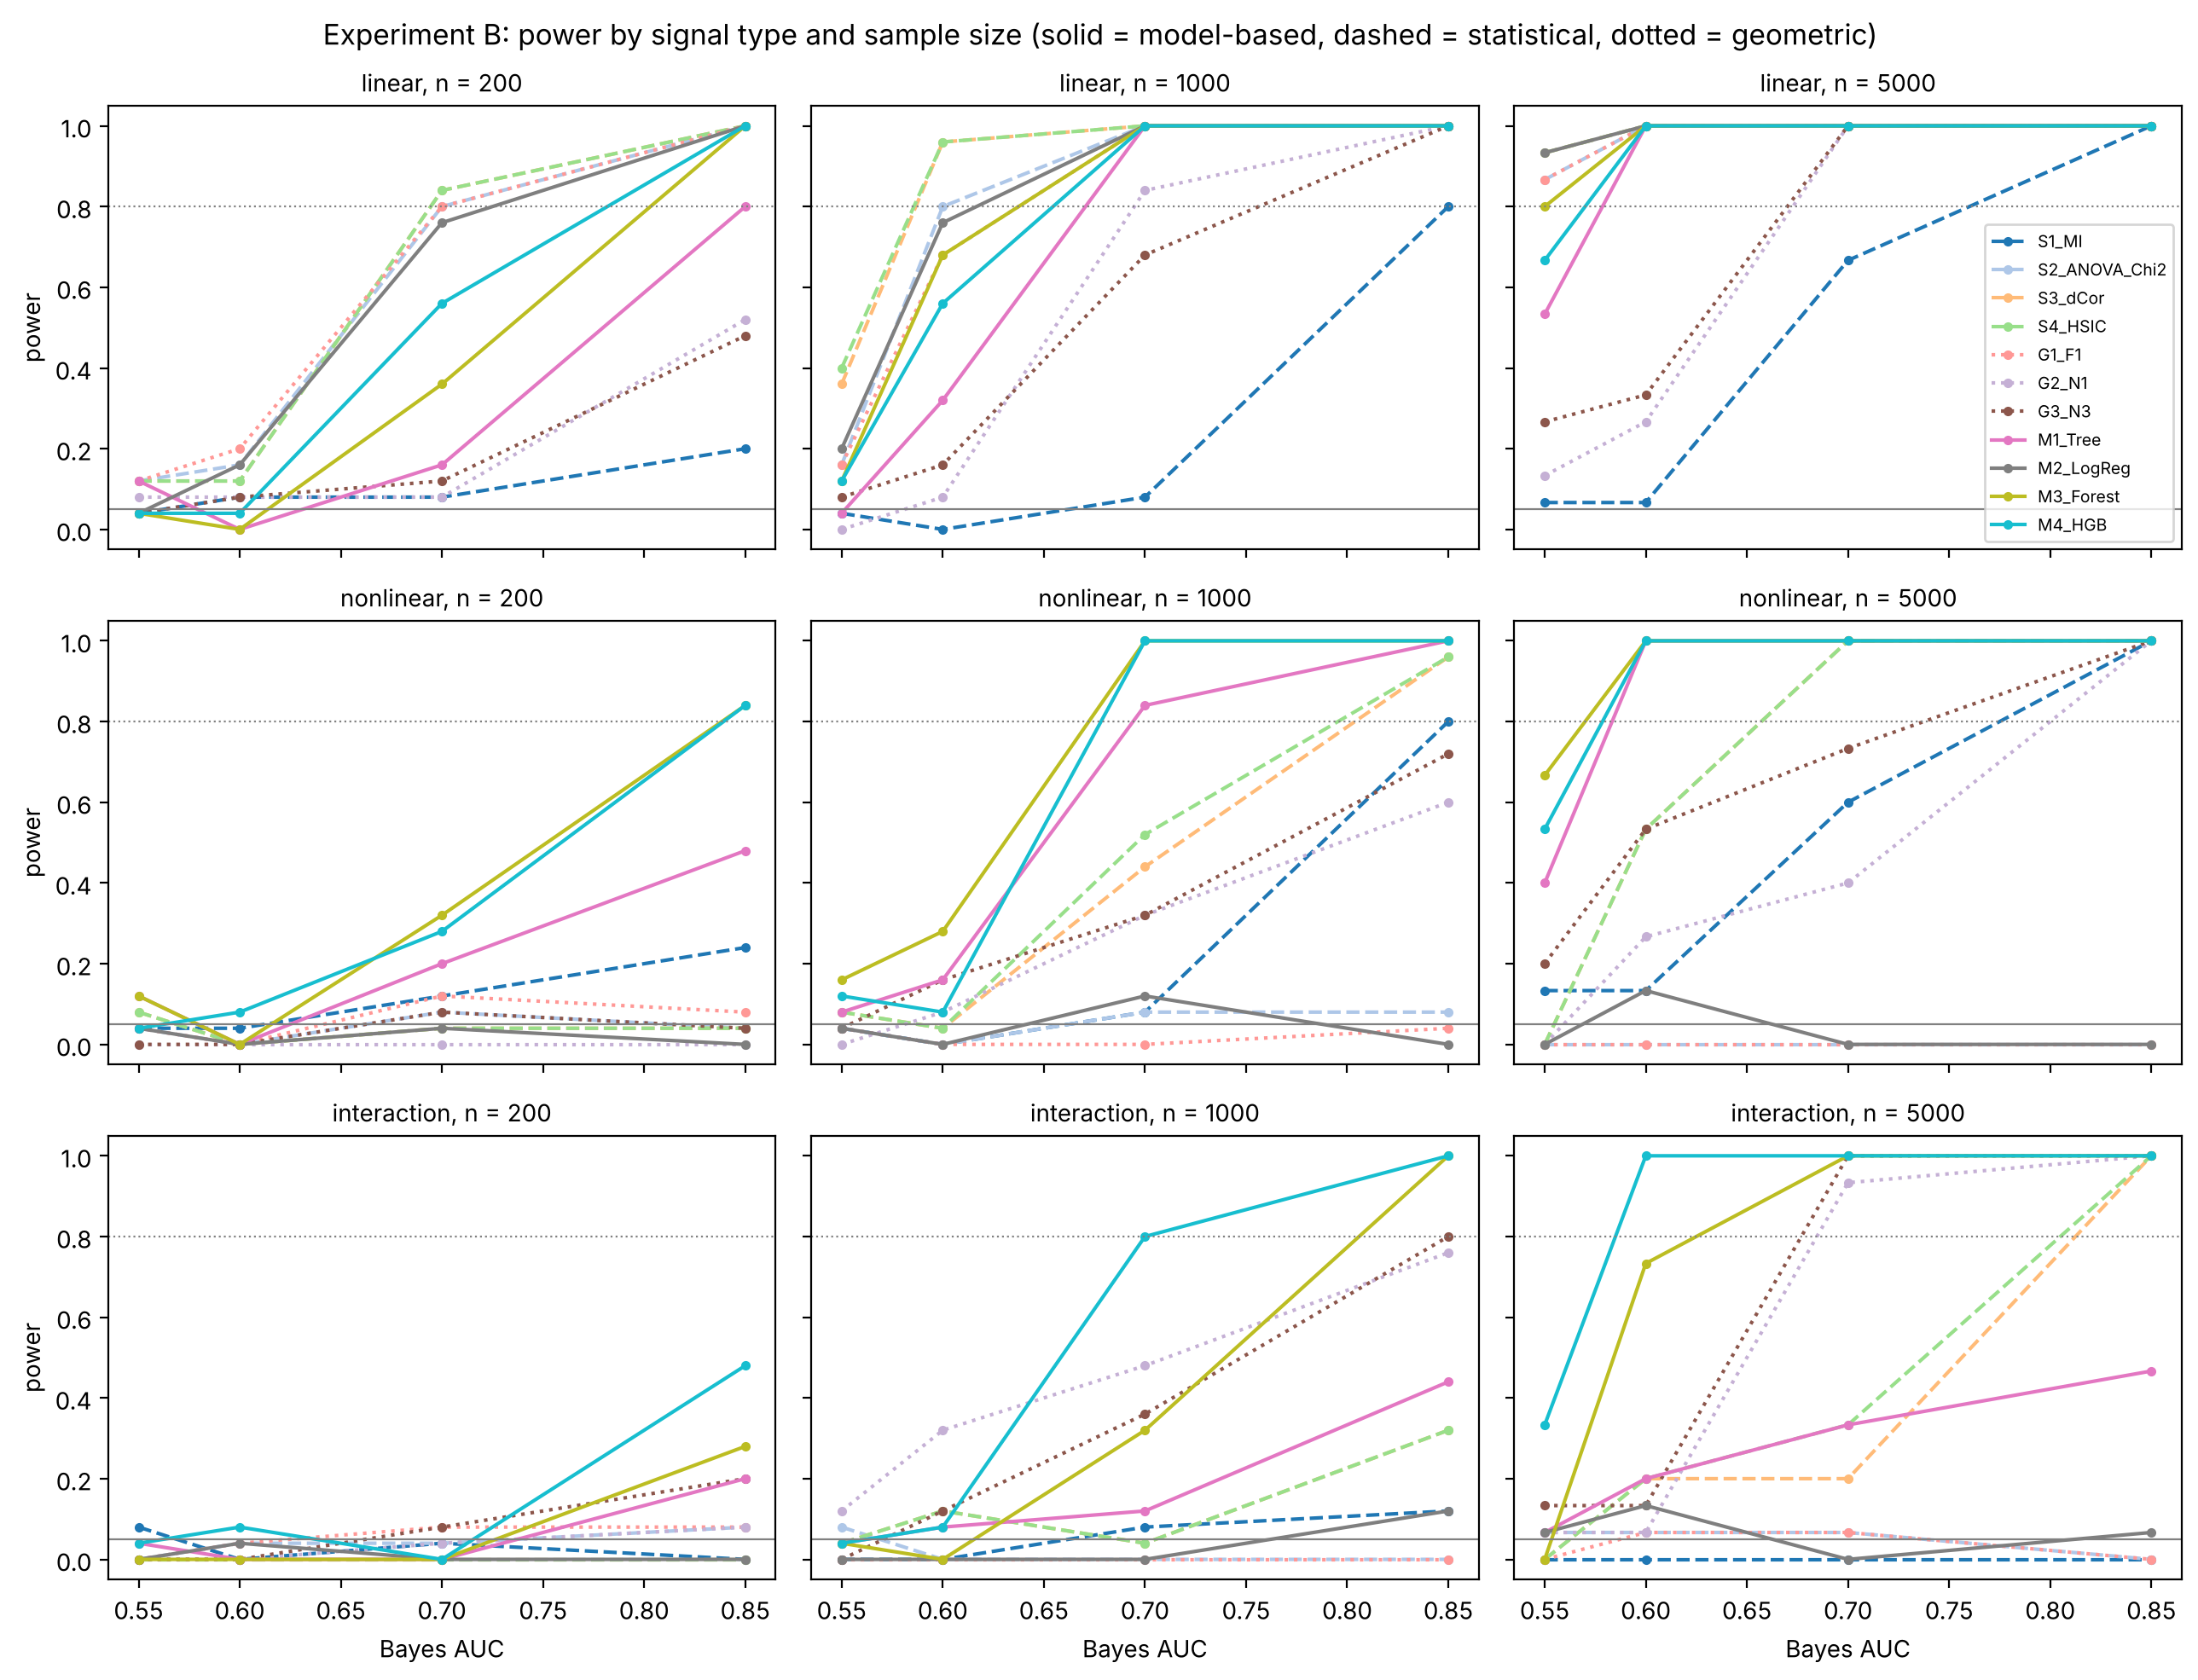
\includegraphics[width=0.92\textwidth]{../figures/expB_power_curves.png}
\caption{Experiment B: power against Bayes AUC by signal type (rows) and sample size (columns). Solid lines: model-based probes; dashed: statistical; dotted: geometric. Grey lines mark $\alpha=0.05$ and 80\% power.}
\label{fig:power}
\end{figure*}

\begin{table*}[!t]
\centering
\caption{Experiment B: mean power at $\alpha=0.05$, averaged over the four signal strengths (Bayes AUC 0.55--0.85).}
\label{tab:power}
\footnotesize
\begin{adjustbox}{max width=\linewidth}
\begin{tabular}{lccccccc}
\hline
Probe & All & Interaction & Linear & Nonlinear & $n$=200 & $n$=1000 & $n$=5000 \\ \hline
S1 MI & 0.19 & 0.03 & 0.26 & 0.27 & 0.08 & 0.17 & 0.31 \\
S2 ANOVA/$\chi^2$ & 0.27 & 0.04 & 0.74 & 0.03 & 0.20 & 0.27 & 0.34 \\
S3 dCor & 0.43 & 0.16 & 0.78 & 0.35 & 0.19 & 0.45 & 0.66 \\
S4 HSIC & 0.44 & 0.17 & 0.78 & 0.36 & 0.19 & 0.46 & 0.67 \\
G1 F1 & 0.26 & 0.03 & 0.74 & 0.03 & 0.21 & 0.24 & 0.33 \\
G2 N1 & 0.32 & 0.32 & 0.42 & 0.22 & 0.07 & 0.38 & 0.51 \\
G3 N3 & 0.36 & 0.32 & 0.44 & 0.32 & 0.09 & 0.37 & 0.61 \\
M1 Tree & 0.42 & 0.17 & 0.58 & 0.52 & 0.18 & 0.43 & 0.67 \\
M2 LogReg & 0.27 & 0.04 & 0.74 & 0.03 & 0.17 & 0.27 & 0.36 \\
M3 Forest & 0.55 & 0.36 & 0.67 & 0.62 & 0.25 & 0.55 & 0.85 \\
M4 HGB & 0.58 & 0.49 & 0.67 & 0.58 & 0.29 & 0.57 & 0.88 \\
\hline
\end{tabular}
\end{adjustbox}
\end{table*}


Across the 36 settings the probes differed strongly (Friedman $\chi^2=65.3$, $p=3.5\times10^{-10}$; Table~\ref{tab:ranks}); following~\cite{benavoli2016}, each probe was then compared with the best one by a Wilcoxon signed-rank test with Holm correction. Gradient boosting had the best mean rank (3.92). The random forest (Holm $p=0.41$), HSIC and distance correlation (both $p=0.091$) were not significantly worse; all other probes were. At $n=200$ every probe had low power (at most 0.29), with gradient boosting highest and F1 the best model-free probe (0.21). H1c is therefore supported in the narrow sense that a model-based probe was most powerful, but no probe is reliable at $n=200$ unless the signal is strong and linear.

\begin{table}[!t]
\centering
\caption{Ranking of probes over the 36 settings of Experiment B (Friedman $\chi^2=65.3$, $p=3.5e-10$). Gap and $p$-value refer to a Wilcoxon signed-rank comparison with the best-ranked probe, Holm-corrected.}
\label{tab:ranks}
\footnotesize
\begin{adjustbox}{max width=\linewidth}
\begin{tabular}{lccc}
\hline
Probe & Mean rank & Power gap to best & Holm $p$ \\ \hline
M4 HGB & 3.92 & -- & -- \\
M3 Forest & 4.54 & 0.029 & 0.406 \\
M1 Tree & 5.10 & 0.155 & 0.002 \\
S4 HSIC & 5.22 & 0.141 & 0.091 \\
S3 dCor & 5.32 & 0.149 & 0.091 \\
G3 N3 & 6.25 & 0.220 & 2.6e-04 \\
S2 ANOVA/$\chi^2$ & 6.61 & 0.309 & 0.009 \\
G1 F1 & 6.85 & 0.315 & 0.008 \\
G2 N1 & 6.97 & 0.256 & 2.8e-04 \\
M2 LogReg & 7.15 & 0.310 & 0.004 \\
S1 MI & 8.07 & 0.393 & 1.4e-05 \\
\hline
\end{tabular}
\end{adjustbox}
\end{table}


\begin{table*}[!t]
\centering
\caption{Minimum detectable effect: smallest Bayes AUC at which a probe reaches 80\% power (linear interpolation; ``$>0.85$'' = never within the tested range).}
\label{tab:mde}
\footnotesize
\begin{adjustbox}{max width=\linewidth}
\begin{tabular}{lccccccccc}
\hline
Probe & inter. 200 & inter. 1000 & inter. 5000 & lin. 200 & lin. 1000 & lin. 5000 & nonli. 200 & nonli. 1000 & nonli. 5000 \\ \hline
S1 MI & $>$0.85 & $>$0.85 & $>$0.85 & $>$0.85 & 0.850 & 0.760 & $>$0.85 & 0.850 & 0.775 \\
S2 ANOVA/$\chi^2$ & $>$0.85 & $>$0.85 & $>$0.85 & 0.700 & 0.600 & $\le$0.55 & $>$0.85 & $>$0.85 & $>$0.85 \\
S3 dCor & $>$0.85 & $>$0.85 & 0.812 & 0.694 & 0.587 & $\le$0.55 & $>$0.85 & 0.804 & 0.657 \\
S4 HSIC & $>$0.85 & $>$0.85 & 0.805 & 0.694 & 0.586 & $\le$0.55 & $>$0.85 & 0.795 & 0.657 \\
G1 F1 & $>$0.85 & $>$0.85 & $>$0.85 & 0.700 & 0.637 & $\le$0.55 & $>$0.85 & $>$0.85 & $>$0.85 \\
G2 N1 & $>$0.85 & $>$0.85 & 0.685 & $>$0.85 & 0.695 & 0.673 & $>$0.85 & $>$0.85 & 0.800 \\
G3 N3 & $>$0.85 & 0.850 & 0.677 & $>$0.85 & 0.756 & 0.670 & $>$0.85 & $>$0.85 & 0.738 \\
M1 Tree & $>$0.85 & $>$0.85 & $>$0.85 & 0.850 & 0.671 & 0.579 & $>$0.85 & 0.694 & 0.583 \\
M2 LogReg & $>$0.85 & $>$0.85 & $>$0.85 & 0.725 & 0.617 & $\le$0.55 & $>$0.85 & $>$0.85 & $>$0.85 \\
M3 Forest & $>$0.85 & 0.806 & 0.625 & 0.803 & 0.637 & $\le$0.55 & 0.838 & 0.672 & 0.570 \\
M4 HGB & $>$0.85 & 0.700 & 0.585 & 0.782 & 0.655 & 0.570 & 0.839 & 0.678 & 0.579 \\
\hline
\end{tabular}
\end{adjustbox}
\end{table*}


\subsection{Robustness (RQ2: H2b, H2c)}

Irrelevant features hurt the distance-based probes most (Table~\ref{tab:robust}). With balanced classes, power at Bayes AUC 0.70 fell from 0.99 to 0.35 for distance correlation, from 1.00 to 0.35 for HSIC, from 0.99 to 0.13 for N1 and from 0.88 to 0.08 for N3 as irrelevant features went from 0 to 200, an average drop of 0.74. The model-based probes fell by 0.29 on average (forest 1.00 to 0.60, gradient boosting 1.00 to 0.65), supporting H2b and agreeing with the known dimension sensitivity of distance- and kernel-based tests~\cite{ramdas2015}. Under 10\% positives, permutation tests stayed calibrated (largest pooled FPR 0.058), and the forest remained the most powerful probe (0.93, 0.75 and 0.44 for 0, 20 and 200 irrelevant features). The geometric neighbourhood measures were the most affected by imbalance (N1: 0.23 with no irrelevant features). H2c is supported.

\begin{table}[!t]
\centering
\caption{Experiment C: power at Bayes AUC 0.70 and $n=1000$, averaged over the three signal types, by number of irrelevant features. Left block: balanced classes; right block: 10\% positives.}
\label{tab:robust}
\footnotesize
\begin{adjustbox}{max width=\linewidth}
\begin{tabular}{lcccccc}
\hline
Probe & 0 & 20 & 200 & 0  & 20  & 200  \\ \hline
S1 MI & 0.35 & 0.08 & 0.04 & 0.33 & 0.09 & 0.07 \\
S2 ANOVA/$\chi^2$ & 0.36 & 0.36 & 0.35 & 0.44 & 0.37 & 0.29 \\
S3 dCor & 0.99 & 0.49 & 0.35 & 0.77 & 0.47 & 0.37 \\
S4 HSIC & 1.00 & 0.52 & 0.35 & 0.79 & 0.49 & 0.24 \\
G1 F1 & 0.39 & 0.33 & 0.35 & 0.44 & 0.36 & 0.25 \\
G2 N1 & 0.99 & 0.55 & 0.13 & 0.23 & 0.08 & 0.07 \\
G3 N3 & 0.88 & 0.45 & 0.08 & 0.28 & 0.09 & 0.04 \\
M1 Tree & 0.84 & 0.65 & 0.48 & 0.41 & 0.53 & 0.41 \\
M2 LogReg & 0.40 & 0.37 & 0.35 & 0.39 & 0.35 & 0.23 \\
M3 Forest & 1.00 & 0.77 & 0.60 & 0.93 & 0.75 & 0.44 \\
M4 HGB & 1.00 & 0.93 & 0.65 & 0.76 & 0.59 & 0.25 \\
\hline
\end{tabular}
\end{adjustbox}
\end{table}


\subsection{Cost (RQ3: H3)}

On Adult subsamples (Table~\ref{tab:runtime}), one observed statistic cost 0.007--0.23~s for F1, N3, S1, S2 and the tree, about 2~s for distance correlation, HSIC and the forest, 9~s for N1 (dominated by the minimum spanning tree) and 7.5~s for gradient boosting, against 20.2~s for one 5-fold cross-validation of gradient boosting on all 48{,}842 rows. Because model-free probes reuse their label-independent preparation, their complete permutation test with $B=200$ took 0.2--28.5~s; a model-based test costs roughly $(B+1)$ times one cross-validation. At $n=5000$, S2, F1, the tree, the forest and gradient boosting were Pareto-optimal in power versus cost. A model-free probe is thus on the front, but power for $n\ge10{,}000$ was not simulated, so H3 is only partly supported.

\begin{table*}[!t]
\centering
\caption{Wall-clock seconds for one observed statistic on Adult subsamples (2 CPU cores). Quadratic-cost probes use at most 5{,}000 rows and model-based probes at most 10{,}000.}
\label{tab:runtime}
\footnotesize
\begin{adjustbox}{max width=\linewidth}
\begin{tabular}{lccccc}
\hline
Probe & $n$=1,000 & $n$=5,000 & $n$=10,000 & $n$=20,000 & $n$=48,842 \\ \hline
S1 MI & 0.050 & 0.139 & 0.128 & 0.131 & 0.132 \\
S2 ANOVA/$\chi^2$ & 0.065 & 0.074 & 0.090 & 0.106 & 0.157 \\
S3 dCor & 0.071 & 1.839 & 1.770 & 2.106 & 1.956 \\
S4 HSIC & 0.085 & 1.736 & 1.927 & 2.025 & 1.800 \\
G1 F1 & 0.002 & 0.021 & 0.014 & 0.016 & 0.007 \\
G2 N1 & 0.248 & 9.304 & 9.418 & 10.198 & 8.996 \\
G3 N3 & 0.025 & 0.224 & 0.248 & 0.230 & 0.232 \\
M1 Tree & 0.025 & 0.086 & 0.158 & 0.158 & 0.174 \\
M2 LogReg & 0.102 & 0.382 & 0.632 & 0.642 & 0.629 \\
M3 Forest & 0.513 & 1.042 & 2.289 & 2.160 & 2.063 \\
M4 HGB & 2.626 & 4.929 & 7.064 & 6.823 & 7.492 \\
Ref.: HGB 5-fold CV & 2.472 & 5.033 & 7.219 & 8.573 & 20.196 \\
\hline
\end{tabular}
\end{adjustbox}
\end{table*}


\subsection{Real Distributions (RQ4: H4a, H4b)}

On the label-shuffled real datasets (Fig.~\ref{fig:semi}), every probe detected signal when at most half of the labels were shuffled. At $q=0.9$, distance correlation and HSIC still detected it in 62\% of replicates, S2 and F1 in about 40\%, and gradient boosting in 12\%. The signal in these four datasets is largely monotone in single features, which favours the dependence tests. At $q=1$ (exact null) the detection rate was 0--0.125 per probe (gradient boosting 5 of 40). All probe statistics tracked the retained signal fraction closely (mean Spearman $\rho$: statistical 0.960, model-based 0.953, geometric 0.940). The difference H4a predicted exists but is negligible, so H4a is only nominally supported.

\begin{figure*}[!t]
\centering
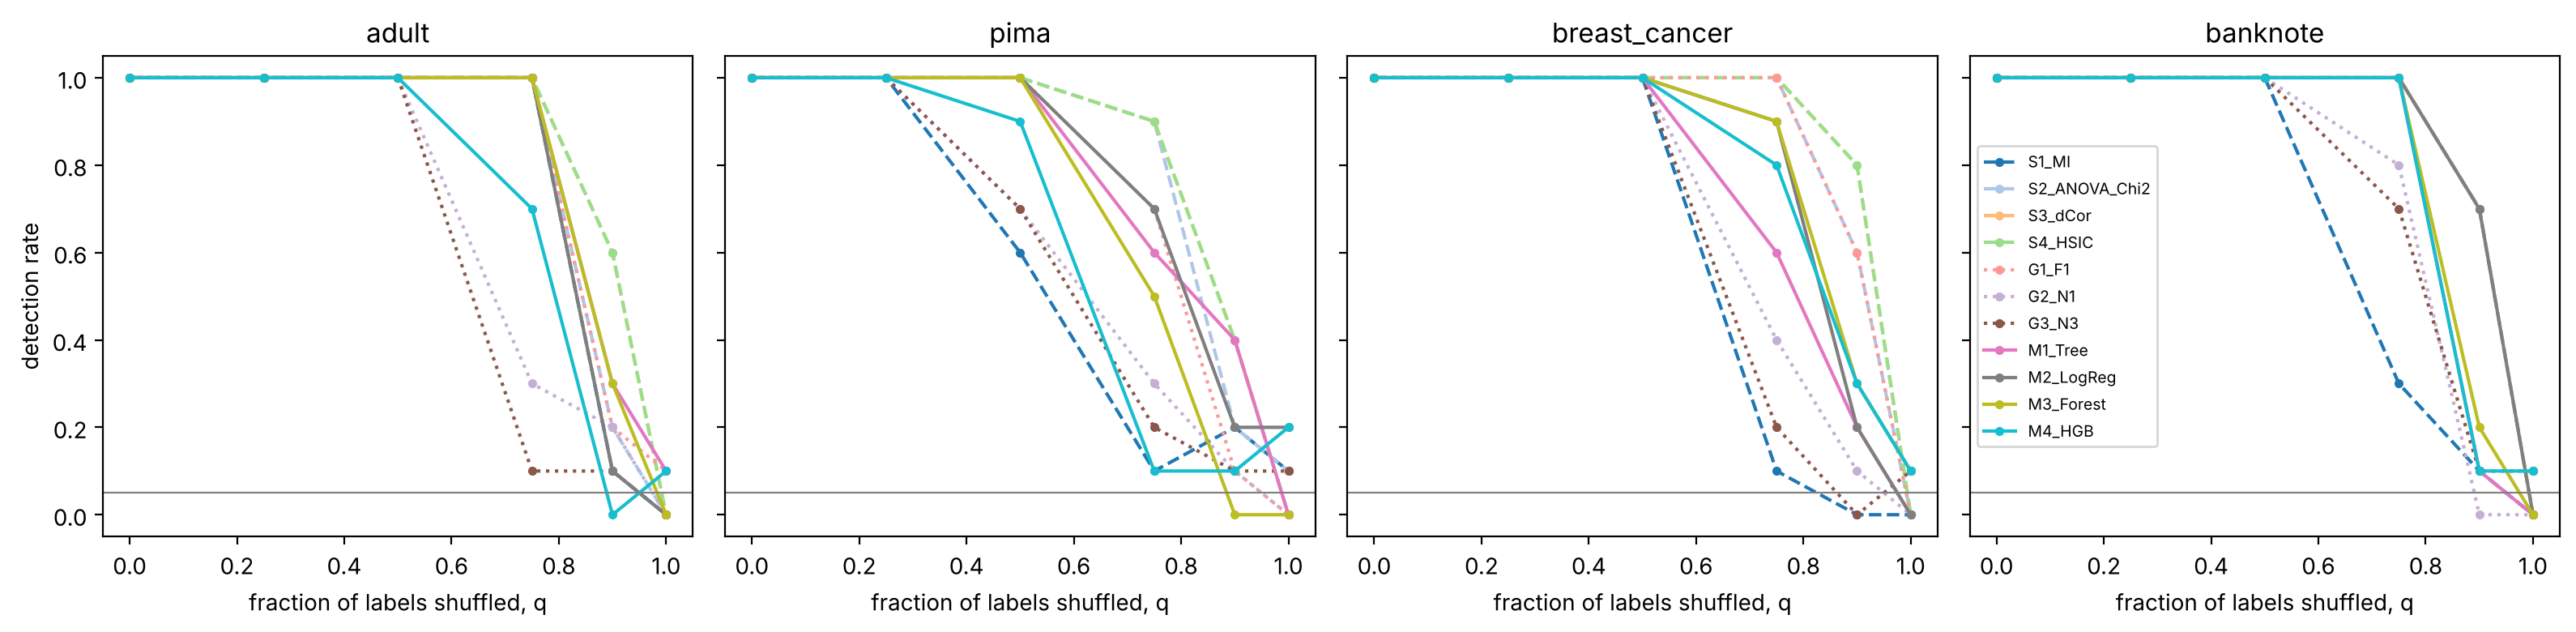
\includegraphics[width=0.95\textwidth]{../figures/semisynthetic_detection.png}
\caption{Semi-synthetic experiment: detection rate against the fraction $q$ of shuffled labels for each base dataset (10 replicates per point). At $q=1$ the labels are fully permuted, so the detection rate is the false-positive rate.}
\label{fig:semi}
\end{figure*}

Selected on Experiment~B alone, the two-stage protocol used HSIC (stage~1) and gradient boosting (stage~2). In Experiment~B its power was 0.519, slightly below gradient boosting alone (0.532), with a hold-out FPR of 0.027. On the semi-synthetic validation data its power was 0.890, well above gradient boosting (0.750) but below HSIC alone (0.920), with no false positives in 40 null replicates. The protocol therefore offers robustness to signal type rather than the highest power in any single scenario, and H4b is partly supported.

\subsection{Case Studies}

Table~\ref{tab:cases} reports every probe on the real datasets. On \textbf{Adult}, all probes rejected $H_0$ at their smallest attainable $p$-value, and the AUC gain over the dummy model on the full data was 0.428 for gradient boosting (95\% interval 0.428--0.429; AUC 0.928) and 0.405 for logistic regression. Learning curves showed logistic regression saturating at about 0.905 from 1{,}000 rows, while gradient boosting kept improving to 0.928, so additional data mainly benefits flexible models.

\begin{table*}[!t]
\centering
\caption{Case studies: permutation $p$-values of every probe (Adult: $B=200$, 40 for M3/M4; NSW: $B=1000$, 200; incentive experiment: $B=500$, 200).}
\label{tab:cases}
\footnotesize
\begin{adjustbox}{max width=\linewidth}
\begin{tabular}{lcccc}
\hline
Probe & Adult & NSW (randomised) & Thornton (randomised) & Thornton incl. village \\ \hline
S1 MI & 0.005 & 0.024 & 0.006 & 0.004 \\
S2 ANOVA/$\chi^2$ & $<$0.001 & 0.017 & 0.106 & $<$0.001 \\
S3 dCor & 0.005 & 0.019 & 0.032 & 0.002 \\
S4 HSIC & 0.005 & 0.036 & 0.026 & 0.002 \\
G1 F1 & 0.005 & 0.011 & 0.106 & 0.002 \\
G2 N1 & 0.005 & 0.901 & 0.162 & 0.002 \\
G3 N3 & 0.005 & 0.515 & 0.495 & 0.002 \\
M1 Tree & 0.005 & 0.027 & 0.012 & 0.010 \\
M2 LogReg & 0.005 & 0.033 & 0.038 & 0.002 \\
M3 Forest & 0.024 & 0.010 & 0.010 & 0.005 \\
M4 HGB & 0.024 & 0.368 & 0.005 & 0.005 \\
\hline
\end{tabular}
\end{adjustbox}
\end{table*}


The two \textbf{randomised experiments} were the most instructive cases. On \textbf{NSW}, eight of the eleven probes gave $p<0.05$, although the protocol's two stages did not reach $\alpha/2$ (HSIC $p=0.036$, gradient boosting $p=0.368$), so the protocol returned ``no signal detected''. The per-feature test traced the dependence to the no-degree indicator ($p=0.0021$, the only feature rejected by Benjamini--Hochberg; standardised mean difference $-0.30$). This is a chance imbalance in the subsample rather than a design feature, and the cross-validated AUC gains were small (logistic regression 0.056).

On the \textbf{incentive experiment} with individual covariates only, gradient boosting ($p=0.005$, AUC gain 0.058) and the forest ($p=0.010$) detected dependence, and the protocol returned ``signal detected''. With village included, every probe rejected $H_0$ ($p\le0.01$; logistic-regression gain 0.177). Two diagnostics explain part of this. Distance alone identified a person's village with 44\% accuracy, against 4.4\% for the most common village. Under a design-aware test that permutes labels only within villages, distance correlation was no longer significant ($p=0.35$, against 0.025 under ordinary permutation). The tree ensembles, however, stayed significant (forest $p=0.035$, gradient boosting $p=0.015$), which points to further design structure that the public data do not document. In short, ``null by design'' is a claim about the design, and the probes found that it did not hold exactly in either randomised dataset.

\subsection{Ojala--Garriga Replication}

Table~\ref{tab:ojala} and Fig.~\ref{fig:ojala} summarise both tests. Test~1 was significant ($p=0.005$, the minimum) for all four classifiers on Adult, Pima, Banknote, Breast Cancer and the synthetic linear data, and non-significant for every classifier on Adult with permuted labels ($p\ge0.60$), NSW ($p\ge0.06$) and the incentive experiment with individual covariates ($p\ge0.10$). The interaction-only data separated the classifiers: the unpruned tree ($p=0.25$) and naive Bayes ($p=0.82$) missed the signal, whereas 1-NN ($p=0.035$) and the SVM ($p=0.005$) detected it. For exactly those two, Test~2 was also significant ($p=0.005$), correctly identifying that their signal lies in a dependency between features. Test~2 was also significant for the tree, 1-NN and SVM on Banknote, but not on Adult, Pima or Breast Cancer, where within-class permutation did not increase the error ($p\ge0.84$), consistent with signal carried by individual features.

\begin{table*}[!t]
\centering
\caption{Ojala--Garriga replication: accuracy / Test~1 $p$ / Test~2 $p$ per classifier (10-fold CV, $k=200$ permutations; smallest attainable $p$ = 0.005).}
\label{tab:ojala}
\footnotesize
\begin{adjustbox}{max width=\linewidth}
\begin{tabular}{lcccc}
\hline
Dataset & DT & NB & 1NN & SVM \\ \hline
Adult (n=2000) & 0.81 / 0.005 / 1.000 & 0.33 / 0.005 / 1.000 & 0.79 / 0.005 / 1.000 & 0.85 / 0.005 / 1.000 \\
Pima & 0.70 / 0.005 / 0.920 & 0.76 / 0.005 / 1.000 & 0.71 / 0.005 / 0.846 & 0.76 / 0.005 / 1.000 \\
Banknote & 0.99 / 0.005 / 0.005 & 0.84 / 0.005 / 1.000 & 1.00 / 0.005 / 0.005 & 1.00 / 0.005 / 0.005 \\
Breast cancer & 0.92 / 0.005 / 1.000 & 0.94 / 0.005 / 1.000 & 0.95 / 0.005 / 1.000 & 0.98 / 0.005 / 1.000 \\
Synthetic linear & 0.61 / 0.005 / 0.075 & 0.70 / 0.005 / 0.398 & 0.60 / 0.005 / 0.219 & 0.68 / 0.005 / 0.458 \\
Synthetic interaction & 0.51 / 0.249 / 0.383 & 0.48 / 0.821 / 0.965 & 0.54 / 0.035 / 0.005 & 0.64 / 0.005 / 0.005 \\
NSW (randomised) & 0.51 / 0.667 / 0.876 & 0.58 / 0.070 / 0.318 & 0.51 / 0.597 / 0.776 & 0.60 / 0.060 / 0.468 \\
Thornton (randomised) & 0.65 / 0.100 / 0.806 & 0.77 / 0.572 / 1.000 & 0.65 / 0.100 / 0.308 & 0.77 / 0.866 / 0.915 \\
Adult, permuted labels & 0.62 / 0.791 / 0.746 & 0.25 / 0.851 / 0.239 & 0.63 / 0.607 / 0.627 & 0.76 / 0.851 / 0.995 \\
Thornton incl. village & 0.68 / 0.005 / 0.597 & 0.34 / 0.015 / 0.915 & 0.68 / 0.005 / 0.453 & 0.76 / 0.905 / 0.592 \\
\hline
\end{tabular}
\end{adjustbox}
\end{table*}


\begin{figure*}[!t]
\centering
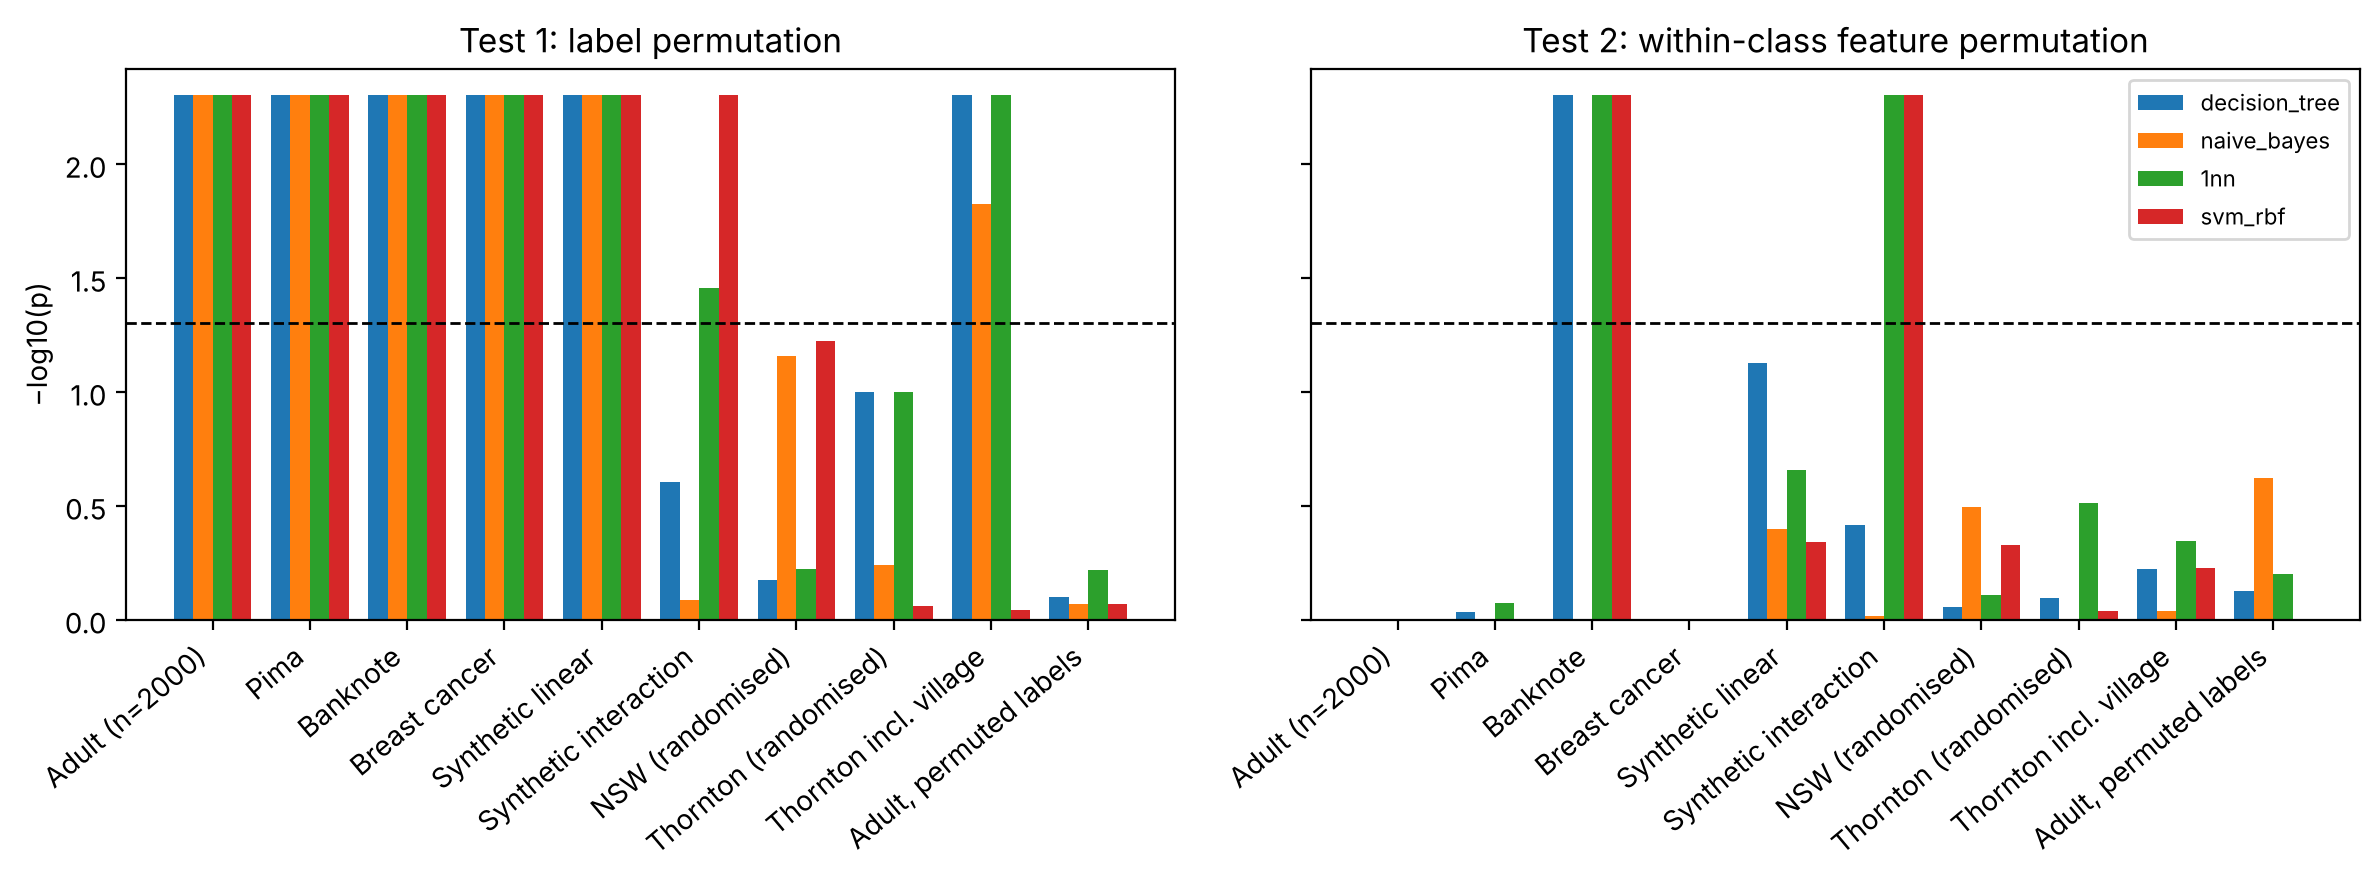
\includegraphics[width=0.92\textwidth]{../figures/ojala_garriga.png}
\caption{Ojala--Garriga Tests 1 and 2: $-\log_{10}p$ per classifier and dataset ($k=200$ permutations; ceiling 2.3). Dashed line: $p=0.05$.}
\label{fig:ojala}
\end{figure*}

Accuracy-based Test~1 and the AUC-based model probes disagreed on the incentive experiment (77\% positives): no classifier's accuracy beat its permutation distribution, whereas gradient boosting's AUC did ($p=0.005$). Under imbalance, accuracy is dominated by the majority class, so AUC is the more sensitive statistic.

\subsection{Leakage}

The sanity check (Table~\ref{tab:sanity}) flagged the identifier column, the crude leak (single-feature AUC 0.995) and the incentive amount in the incentive experiment (AUC 1.000). It passed the subtle leak (a copy of $y$ with 10\% flipped values, AUC 0.90), on which every probe rejected $H_0$ ($p\le0.026$), and it passed NSW with the post-treatment earnings \texttt{re78}. A clean sanity check is therefore no guarantee: post-outcome features must be excluded by reasoning about when each variable was measured.

\begin{table}[!t]
\centering
\caption{Experiment D: sanity check verdicts.}
\label{tab:sanity}
\footnotesize
\begin{adjustbox}{max width=\linewidth}
\begin{tabular}{llcc}
\hline
Case & Sanity verdict & Best single feature & Its AUC \\ \hline
Null synthetic (control) & clean & x7 & 0.543 \\
Null + identifier column & leakage suspected & x7 & 0.543 \\
Null + crude leak (0.5\% flipped copy of y) & leakage suspected & leak & 0.995 \\
Null + subtle leak (10\% flipped copy of y) & clean & leak & 0.900 \\
NSW pre-treatment only & clean & nodegree & 0.563 \\
NSW + re78 (post-treatment) & clean & re78 & 0.570 \\
Thornton pre-treatment only & clean & age & 0.523 \\
Thornton + village & clean & villnum & 0.659 \\
Thornton + tinc (incentive amount) & leakage suspected & tinc & 1.000 \\
Adult & clean & relationship & 0.778 \\
Pima & clean & glucose & 0.788 \\
Banknote & clean & variance & 0.927 \\
Breast cancer & clean & worst\_perimeter & 0.975 \\
\hline
\end{tabular}
\end{adjustbox}
\end{table}


\FloatBarrier
\section{Discussion}
\label{sec:discussion}

Table~\ref{tab:verdicts} summarises the hypothesis verdicts. Four findings matter most for practice.

\textbf{No single family is sufficient.} Linear dependence tests (S2, F1, logistic regression) are efficient for additive signal but blind to signal that changes spread or lives in interactions, and the latter is exactly where flexible learners are needed. Distance correlation and HSIC are the best model-free compromise, but they degrade quickly with irrelevant features. Gradient boosting had the best overall rank, yet on the real, largely monotone datasets it was the least powerful model-based probe. Pairing a multivariate dependence test with a flexible learner is therefore a reasonable default, and Ojala--Garriga's Test~2 adds a cheap diagnostic of \emph{where} the signal lives.

\textbf{Calibration is easy; aggregation and resolution are not.} Permutation wrapping made every probe's false-positive rate exact, including the descriptive complexity measures, which have no null distribution of their own (gap G2). The two practical traps are combining per-feature tests without correction, which raised the FPR to 0.90 with 50 features, and using too few permutations for a per-feature test, which made S1 unable to reject at all.

\textbf{Small samples are the hard case.} At $n=200$ no probe exceeded 0.29 mean power, and most signals with Bayes AUC below 0.7 went undetected. A ``no signal detected'' verdict at that size says little unless it carries the MDE: for example, gradient boosting at $n=1000$ detects interaction signal only above a Bayes AUC of about 0.70.

\textbf{``No signal by design'' must be verified.} Both randomised experiments carried detectable dependence: a chance covariate imbalance in NSW, and assignment probabilities that varied by village in the incentive experiment. The probes behaved correctly; the assumption was wrong. For practitioners this cuts both ways: a probe that rejects $H_0$ shows that the target depends on the features in \emph{this sample}, which is not the same as stable, useful signal. Effect sizes (NSW: AUC gain about 0.05) and design-aware nulls such as within-stratum permutation should accompany the verdict.

\begin{table}[!t]
\centering
\caption{Verdicts on the pre-registered hypotheses.}
\label{tab:verdicts}
\footnotesize
\begin{adjustbox}{max width=\linewidth}
\begin{tabular}{lp{5.3cm}l}
\hline
Hypothesis & Statement & Verdict \\ \hline
H1a & Permutation-wrapped probes are calibrated & supported \\
H1b & Uncorrected per-feature aggregation inflates FPR; Simes/BH restores it & supported \\
H1c & Model-based probes most powerful at small n & supported \\
H2a & Per-feature probes blind to interaction-only signal & supported \\
H2b & Distance-based probes lose power faster with irrelevant features & supported \\
H2c & AUC-based probes stay calibrated and useful under 10:90 imbalance & supported \\
H3 & A model-free probe is Pareto-optimal at large n & partly supported \\
H4a & Model-based effect sizes track true strength better than geometric scores & nominal only (difference $<$ 0.02) \\
H4b & Two-stage protocol $\ge$ best single probe in power with FPR $\le$ $\alpha$ & partly supported \\
\hline
\end{tabular}
\end{adjustbox}
\end{table}


\textbf{Limitations.} Compute restrictions (two CPU cores, no GPU, GitHub-only network access) forced three deviations from the proposal: a random forest replaced TabPFN, scikit-learn's histogram gradient boosting replaced LightGBM, and power was simulated only up to $n=5000$ with 15--25 replicates per setting, which gives power estimates a standard error of up to 0.1. Synthetic features were Gaussian, so the categorical and mixed-type behaviour of the probes was tested only on the real datasets. Only binary targets and exchangeable rows were considered. Finally, the protocol's stages were selected on synthetic data whose signal types differ from those in the real datasets, which explains part of the gap between design and validation power.

\section{Conclusion}
\label{sec:conclusion}

Whether a tabular dataset holds learnable signal can be tested cheaply and with exact error control by wrapping statistical, geometric or model-based probes in a shared permutation layer. Across controlled, semi-synthetic and real data, the probes' power depended mainly on the type of signal: dependence tests excelled at linear signal, flexible learners at nonlinear and interaction signal, and neighbourhood complexity measures were sensitive to irrelevant features. A two-stage protocol (HSIC, then gradient boosting, Bonferroni-split) kept the false-positive rate below $\alpha$ and was robust across signal types, though not the most powerful choice in every scenario. The replication of Ojala and Garriga's tests showed that Test~2 reliably reveals interaction signal. Datasets that were null by design, finally, turned out not to be null in the sample, a reminder that the verdict ``signal detected'' always needs an effect size and a check of the design behind the data. Future work should add tabular foundation models, regression targets and power estimates for $n>5000$.


\section*{Data and Code Availability}
All datasets are public. The eight Jupyter notebooks that download the data, implement every probe, run all experiments and generate every table and figure in this paper accompany the submission.

\section*{Use of AI Tools}
[To be completed by the author in line with the university's rules on independent work, describing which AI tools were used and for which tasks.]

\FloatBarrier
\begin{thebibliography}{48}
\bibitem{grinsztajn2022}
L.~Grinsztajn, E.~Oyallon, and G.~Varoquaux, ``Why do tree-based models still outperform deep learning on typical tabular data?,'' in \emph{Adv. Neural Inf. Process. Syst. (NeurIPS), Datasets and Benchmarks Track}, vol.~35, 2022.

\bibitem{erickson2025}
N.~Erickson \emph{et al.}, ``TabArena: A living benchmark for machine learning on tabular data,'' in \emph{Adv. Neural Inf. Process. Syst. (NeurIPS), Datasets and Benchmarks Track}, 2025, arXiv:2506.16791.

\bibitem{hollmann2025}
N.~Hollmann \emph{et al.}, ``Accurate predictions on small data with a tabular foundation model,'' \emph{Nature}, vol.~637, no.~8045, pp.~319--326, 2025, doi: 10.1038/s41586-024-08328-6.

\bibitem{renggli2020snoopy}
C.~Renggli \emph{et al.}, ``Ease.ml/snoopy in action: Towards automatic feasibility analysis for machine learning application development,'' \emph{Proc. VLDB Endow.}, vol.~13, no.~12, pp.~2837--2840, 2020.

\bibitem{renggli2023feasibility}
C.~Renggli \emph{et al.}, ``Automatic feasibility study via data quality analysis for ML: A case-study on label noise,'' in \emph{Proc. IEEE Int. Conf. Data Eng. (ICDE)}, 2023, arXiv:2010.08410.

\bibitem{lorena2019}
A.~C. Lorena, L.~P.~F. Garcia, J.~Lehmann, M.~C.~P. Souto, and T.~K. Ho, ``How complex is your classification problem? A survey on measuring classification complexity,'' \emph{ACM Comput. Surv.}, vol.~52, no.~5, Art. no.~107, 2019.

\bibitem{ross2014}
B.~C. Ross, ``Mutual information between discrete and continuous data sets,'' \emph{PLoS ONE}, vol.~9, no.~2, Art. no.~e87357, 2014.

\bibitem{ojala2010}
M.~Ojala and G.~C. Garriga, ``Permutation tests for studying classifier performance,'' \emph{J. Mach. Learn. Res.}, vol.~11, pp.~1833--1863, 2010.

\bibitem{varoquaux2018}
G.~Varoquaux, ``Cross-validation failure: Small sample sizes lead to large error bars,'' \emph{NeuroImage}, vol.~180, pp.~68--77, 2018.

\bibitem{korthauer2019}
K.~Korthauer \emph{et al.}, ``A practical guide to methods controlling false discoveries in computational biology,'' \emph{Genome Biol.}, vol.~20, Art. no.~118, 2019, doi: 10.1186/s13059-019-1716-1.

\bibitem{renggli2021feebee}
C.~Renggli, L.~Rimanic, N.~Hollenstein, and C.~Zhang, ``Evaluating Bayes error estimators on real-world datasets with FeeBee,'' in \emph{Adv. Neural Inf. Process. Syst. (NeurIPS), Datasets and Benchmarks Track}, 2021, arXiv:2108.13034.

\bibitem{theisen2021}
R.~Theisen, H.~Wang, L.~R. Varshney, C.~Xiong, and R.~Socher, ``Evaluating state-of-the-art classification models against Bayes optimality,'' in \emph{Adv. Neural Inf. Process. Syst. (NeurIPS)}, vol.~34, 2021.

\bibitem{ishida2023}
T.~Ishida, I.~Yamane, N.~Charoenphakdee, G.~Niu, and M.~Sugiyama, ``Is the performance of my deep network too good to be true? A direct approach to estimating the Bayes error in binary classification,'' in \emph{Proc. Int. Conf. Learn. Represent. (ICLR)}, 2023.

\bibitem{smith2014}
M.~R. Smith, T.~Martinez, and C.~Giraud-Carrier, ``An instance level analysis of data complexity,'' \emph{Mach. Learn.}, vol.~95, no.~2, pp.~225--256, 2014.

\bibitem{munoz2018}
M.~A. Mu\~{n}oz, L.~Villanova, D.~Baatar, and K.~Smith-Miles, ``Instance spaces for machine learning classification,'' \emph{Mach. Learn.}, vol.~107, 2018.

\bibitem{rivolli2022}
A.~Rivolli, L.~P.~F. Garcia, C.~Soares, J.~Vanschoren, and A.~C.~P.~L.~F. de~Carvalho, ``Meta-features for meta-learning,'' \emph{Knowl.-Based Syst.}, vol.~240, Art. no.~108101, 2022.

\bibitem{komorniczak2022}
J.~Komorniczak and P.~Ksieniewicz, ``problexity -- An open-source Python library for binary classification problem complexity assessment,'' 2022, arXiv:2207.06709.

\bibitem{pedregosa2011}
F.~Pedregosa \emph{et al.}, ``Scikit-learn: Machine learning in Python,'' \emph{J. Mach. Learn. Res.}, vol.~12, pp.~2825--2830, 2011.

\bibitem{gao2017}
W.~Gao, S.~Kannan, S.~Oh, and P.~Viswanath, ``Estimating mutual information for discrete-continuous mixtures,'' in \emph{Adv. Neural Inf. Process. Syst. (NeurIPS)}, vol.~30, 2017.

\bibitem{mcallester2020}
D.~McAllester and K.~Stratos, ``Formal limitations on the measurement of mutual information,'' in \emph{Proc. Int. Conf. Artif. Intell. Stat. (AISTATS)}, PMLR vol.~108, 2020.

\bibitem{czyz2023}
P.~Czy\.{z}, F.~Grabowski, J.~E. Vogt, N.~Beerenwinkel, and A.~Marx, ``Beyond normal: On the evaluation of mutual information estimators,'' in \emph{Adv. Neural Inf. Process. Syst. (NeurIPS)}, vol.~36, 2023.

\bibitem{szekely2013}
G.~J. Sz\'{e}kely and M.~L. Rizzo, ``Energy statistics: A class of statistics based on distances,'' \emph{J. Stat. Plan. Inference}, vol.~143, no.~8, pp.~1249--1272, 2013.

\bibitem{ramoscarreno2023}
C.~Ramos-Carre\~{n}o and J.~L. Torrecilla, ``dcor: Distance correlation and energy statistics in Python,'' \emph{SoftwareX}, vol.~22, Art. no.~101326, 2023.

\bibitem{sejdinovic2013}
D.~Sejdinovic, B.~Sriperumbudur, A.~Gretton, and K.~Fukumizu, ``Equivalence of distance-based and RKHS-based statistics in hypothesis testing,'' \emph{Ann. Stat.}, vol.~41, no.~5, pp.~2263--2291, 2013.

\bibitem{ramdas2015}
A.~Ramdas, S.~J. Reddi, B.~P\'{o}czos, A.~Singh, and L.~Wasserman, ``On the decreasing power of kernel and distance based nonparametric hypothesis tests in high dimensions,'' in \emph{Proc. AAAI Conf. Artif. Intell.}, vol.~29, 2015.

\bibitem{vergara2014}
J.~R. Vergara and P.~A. Est\'{e}vez, ``A review of feature selection methods based on mutual information,'' \emph{Neural Comput. Appl.}, vol.~24, no.~1, pp.~175--186, 2014.

\bibitem{li2017}
J.~Li \emph{et al.}, ``Feature selection: A data perspective,'' \emph{ACM Comput. Surv.}, vol.~50, no.~6, Art. no.~94, 2017.

\bibitem{lopezpaz2017}
D.~Lopez-Paz and M.~Oquab, ``Revisiting classifier two-sample tests,'' in \emph{Proc. Int. Conf. Learn. Represent. (ICLR)}, 2017.

\bibitem{kim2021}
I.~Kim, A.~Ramdas, A.~Singh, and L.~Wasserman, ``Classification accuracy as a proxy for two-sample testing,'' \emph{Ann. Stat.}, vol.~49, no.~1, 2021, doi: 10.1214/20-AOS1962.

\bibitem{hemerik2018}
J.~Hemerik and J.~Goeman, ``Exact testing with random permutations,'' \emph{TEST}, vol.~27, 2018.

\bibitem{phipson2010}
B.~Phipson and G.~K. Smyth, ``Permutation p-values should never be zero: Calculating exact p-values when permutations are randomly drawn,'' \emph{Stat. Appl. Genet. Mol. Biol.}, vol.~9, no.~1, Art. no.~39, 2010.

\bibitem{hollmann2023}
N.~Hollmann, S.~M{\"u}ller, K.~Eggensperger, and F.~Hutter, ``TabPFN: A transformer that solves small tabular classification problems in a second,'' in \emph{Proc. Int. Conf. Learn. Represent. (ICLR)}, 2023.

\bibitem{qu2025}
J.~Qu, D.~Holzm{\"u}ller, G.~Varoquaux, and M.~Le~Morvan, ``TabICL: A tabular foundation model for in-context learning on large data,'' in \emph{Proc. Int. Conf. Mach. Learn. (ICML)}, PMLR vol.~267, 2025.

\bibitem{hegselmann2023}
S.~Hegselmann, A.~Buendia, H.~Lang, M.~Agrawal, X.~Jiang, and D.~Sontag, ``TabLLM: Few-shot classification of tabular data with large language models,'' in \emph{Proc. Int. Conf. Artif. Intell. Stat. (AISTATS)}, 2023.

\bibitem{bordt2024}
S.~Bordt, H.~Nori, V.~Rodrigues, B.~Nushi, and R.~Caruana, ``Elephants never forget: Memorization and learning of tabular data in large language models,'' in \emph{Proc. Conf. Lang. Model. (COLM)}, 2024.

\bibitem{bates2024}
S.~Bates, T.~Hastie, and R.~Tibshirani, ``Cross-validation: What does it estimate and how well does it do it?,'' \emph{J. Amer. Statist. Assoc.}, vol.~119, no.~546, pp.~1434--1445, 2024.

\bibitem{bouthillier2021}
X.~Bouthillier \emph{et al.}, ``Accounting for variance in machine learning benchmarks,'' in \emph{Proc. Mach. Learn. Syst. (MLSys)}, vol.~3, 2021.

\bibitem{mohr2024}
F.~Mohr and J.~N. van~Rijn, ``Learning curves for decision making in supervised machine learning: A survey,'' \emph{Mach. Learn.}, 2024.

\bibitem{viering2023}
T.~Viering and M.~Loog, ``The shape of learning curves: A review,'' \emph{IEEE Trans. Pattern Anal. Mach. Intell.}, 2023.

\bibitem{kaufman2012}
S.~Kaufman, S.~Rosset, C.~Perlich, and O.~Stitelman, ``Leakage in data mining: Formulation, detection, and avoidance,'' \emph{ACM Trans. Knowl. Discov. Data}, vol.~6, no.~4, Art. no.~15, 2012.

\bibitem{kapoor2023}
S.~Kapoor and A.~Narayanan, ``Leakage and the reproducibility crisis in machine-learning-based science,'' \emph{Patterns}, vol.~4, no.~9, 2023.

\bibitem{frenay2014}
B.~Fr\'{e}nay and M.~Verleysen, ``Classification in the presence of label noise: A survey,'' \emph{IEEE Trans. Neural Netw. Learn. Syst.}, vol.~25, no.~5, pp.~845--869, 2014.

\bibitem{xu2020}
Y.~Xu, S.~Zhao, J.~Song, R.~Stewart, and S.~Ermon, ``A theory of usable information under computational constraints,'' in \emph{Proc. Int. Conf. Learn. Represent. (ICLR)}, 2020.

\bibitem{ethayarajh2022}
K.~Ethayarajh, Y.~Choi, and S.~Swayamdipta, ``Understanding dataset difficulty with $\mathcal{V}$-usable information,'' in \emph{Proc. Int. Conf. Mach. Learn. (ICML)}, PMLR vol.~162, 2022.

\bibitem{dua2019}
D.~Dua and C.~Graff, ``UCI Machine Learning Repository,'' Univ. California, Irvine, School Inf. Comput. Sci., 2019. [Online]. Available: http://archive.ics.uci.edu/ml

\bibitem{imbens2015}
G.~W. Imbens, ``Matching methods in practice: Three examples,'' \emph{J. Hum. Resour.}, vol.~50, no.~2, pp.~373--419, 2015.

\bibitem{cunningham2021}
S.~Cunningham, \emph{Causal Inference: The Mixtape}. New Haven, CT, USA: Yale Univ. Press, 2021.

\bibitem{benavoli2016}
A.~Benavoli, G.~Corani, and F.~Mangili, ``Should we really use post-hoc tests based on mean-ranks?,'' \emph{J. Mach. Learn. Res.}, vol.~17, no.~5, pp.~1--10, 2016.

\end{thebibliography}

\end{document}
